\section{Simulation Analysis}\label{section:sim}
 
In this section, the several steps taken using ngspice in order to conduct the simulation of the audio amplifier, as requested, will be described.
In fact, the group proceded as follows:

\begin{enumerate}
\item Design of the circuit, having as a starting point the circuit given by the professor.

\item Verification of the operation of the transistors in the F.A.R mode. The results are shown below.

\begin{table}[ht]
\parbox{.45\linewidth}{
  \centering
  \begin{tabular}{|l|r|}
    \hline    
   Vce & 1.57786\\ \hline
Vbe & 0.682323\\ \hline
Vce greater than Vbe & Correct F.A.R\\ \hline

  \caption{Verification of the F.A.R mode in the NPN transistor}
\end{table}


\begin{table}[ht]
\parbox{.45\linewidth}{
  \centering
  \begin{tabular}{|l|r|}
    \hline    
   Vec & 2.72908\\ \hline
Veb & 0.781397\\ \hline
Vec greater than Veb & Correct F.A.R\\ \hline

  \caption{Verification of the F.A.R mode in the NPN transistor}
\end{table}



\item OP Analysis
     Then, the OP values of the currents and nodal voltages were computed. These are key to calculate the incremental parameters.
     
     \begin{table}[ht]

  \centering
  \begin{tabular}{|l|r|}
    \hline    
    {\bf Name} & {\bf Value [V,A]} \\ \hline
    @c1[i] & 0.000000e+00\\ \hline
@gb[i] & -2.26065e-04\\ \hline
@r1[i] & 2.161572e-04\\ \hline
@r2[i] & -2.26065e-04\\ \hline
@r3[i] & -9.90741e-06\\ \hline
@r4[i] & 1.183330e-03\\ \hline
@r5[i] & -2.26065e-04\\ \hline
@r6[i] & -9.67173e-04\\ \hline
@r7[i] & 9.671730e-04\\ \hline
v(1) & 5.068716e+00\\ \hline
v(2) & 4.843672e+00\\ \hline
v(3) & 4.369060e+00\\ \hline
v(5) & 4.874693e+00\\ \hline
v(6) & 5.579017e+00\\ \hline
v(7) & -1.98076e+00\\ \hline
v(8) & -2.97458e+00\\ \hline
v(9) & -1.98076e+00\\ \hline

  \end{tabular}
  \caption{Simulation nodal voltage results. All variables are expressed in V or A.} 
\end{table}
     
     
  
\item  In the frequency domain, measure of the output voltage gain, using the function .meas as well as the lower and upper cut off frequencies and the bandwidth.


\begin{table}[ht]
\parbox{.45\linewidth}{
  \centering
  \begin{tabular}{|l|r|}
    \hline    
   Gain& 34.0105\\ \hline
Central Frequency& 794.328\\ \hline
Gain deviation&49.8206\\ \hline
Central frequency deviation&205.672\\ \hline

  \caption{Output impedance in KOhm}
    \label{tab:results}
\end{table}


The quantities obtained are desribed in the table \ref{tab:results}. The first conclusion to be taken from the results are that the main goal of the assignment was achieved, since the voltage gain  in the passband is considerable. However, the bandwidth is not as substancial as desired. As so, we conclude the following:

\begin{itemize}

\item The coupling capacitors' main porpuse is to block the DC signals. If studying an incremental model of an audio amplifier, all values that are constant must be eliminated so the transistors are alwaywas fowardly conducting. One of the reasons for the bandwidth obtained to be small is that, these capacitors also cut some low frequencies. These means that the cut off- frequency is high in our circuit. Nevertheless, due to the weight of the cut off frequency in the calculus of the merti, we were able to obtained a good figure of merit.

\item  As studied in the lectures, the resistor Re has the funciton of stabelizing the effect of the temperature in the DC voltage. Howerver, it has also a negative effect on the gain, once it lowers it. In order to solve the problem, a bypass capacitor Ce is placed in parallel with the resistor, so that the capacitor bypasses the resistor. In DC mode, the resistor plays its effect in the temperature. In AC, the resistor will not affect the gain. To sum up, the capacitor is a short-circuit for higher frequencies (AC) and a open-circuit for low frequencies (DC).

\item IC is the most important current in the circuit because it determines gm, and so directly influences the gain. So, after making some calculations, Rc is of extremely importance.



\end{itemize}
First, it is fundamental to understand the effects that the coupling capacitors have on the volt



\begin{figure}[h] \centering
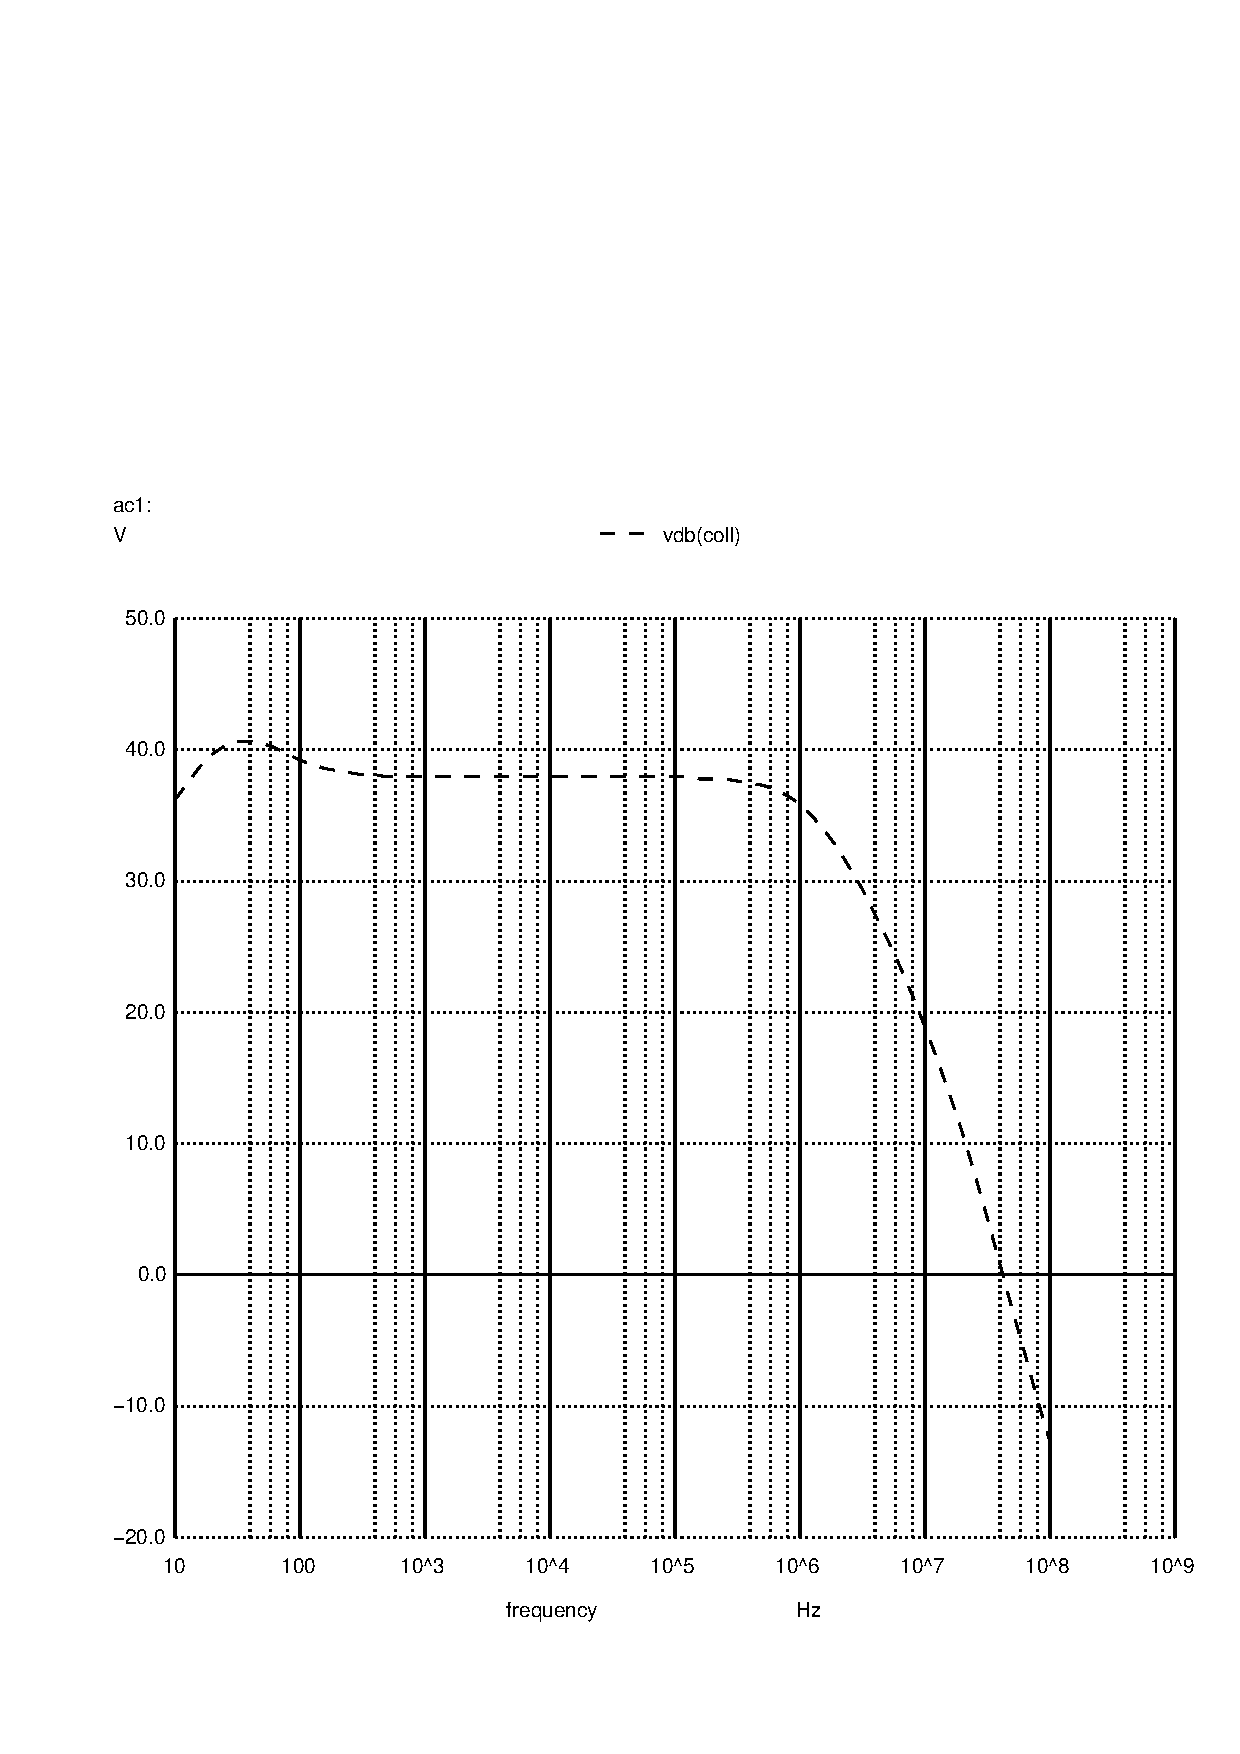
\includegraphics[width=0.4\linewidth]{vo1f.pdf}
\caption{Output voltage of the gain stage}
\label{fig:sim4}
\end{figure}

\begin{figure}[h] \centering
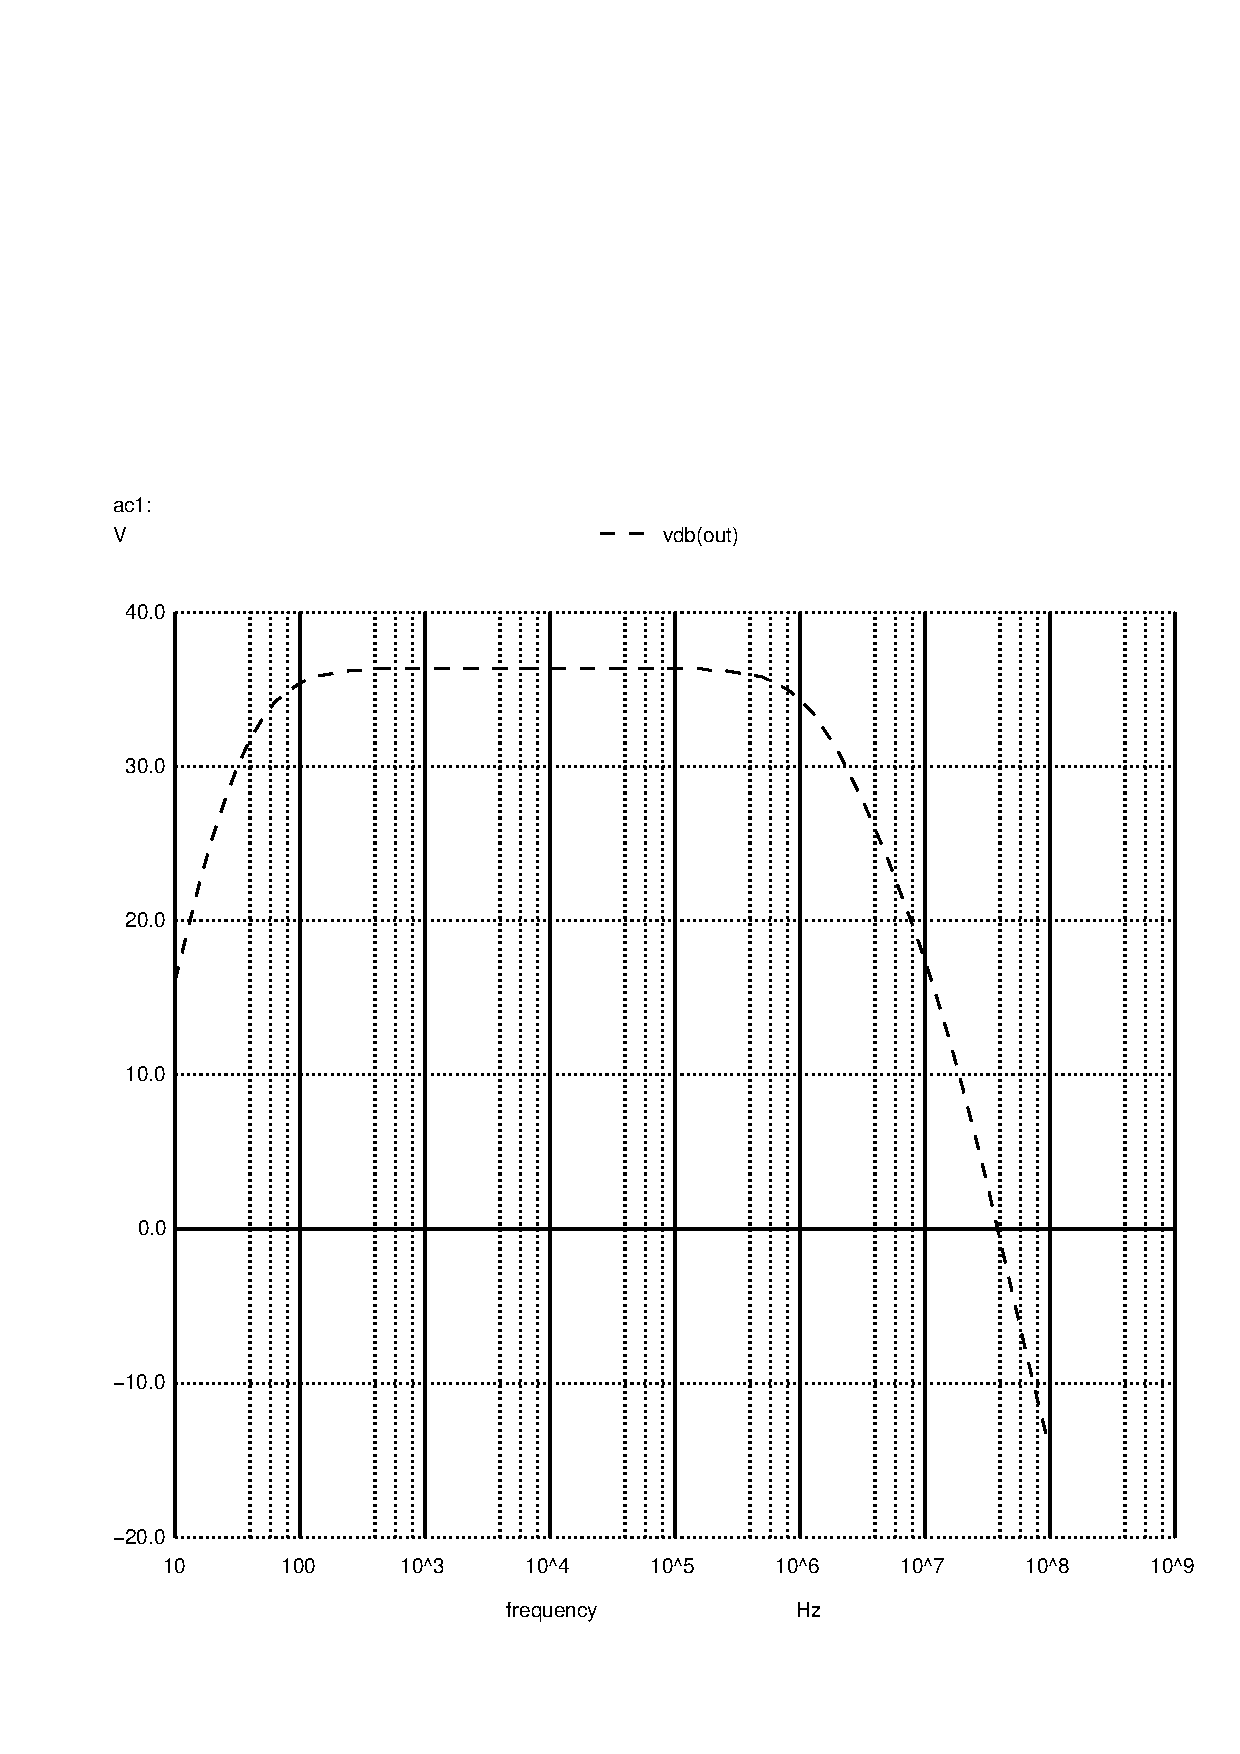
\includegraphics[width=0.4\linewidth]{vo2f.pdf}
\caption{Output voltage of the output stage}
\label{fig:sim4}
\end{figure}






\item Determination of the imput impedance, seen from the imput voltage source.

\begin{table}[ht]
\parbox{.45\linewidth}{
  \centering
  \begin{tabular}{|l|r|}
    \hline    
   Zin & 999.002 + -7.3282 j\\ \hline

  \caption{Output impedance in KOhm}
    \label{tab:ZI}
\end{table}

\par The result obtained for the imput impedance, considering the value in Kohm, is high. Tis is benefitial for the gain, because the voltage in the node In 2 must be as similiar to Vin as possible. Using a voltage dividir, the only way to achieve this was to have a very high resistance value.

\item Determination of the output impedance, using a different set up, seen from the load resistance. 

\begin{table}[ht]
\parbox{.45\linewidth}{
  \centering
  \begin{tabular}{|l|r|}
    \hline    
   Zo & 0.0522978 + -7.23396 j\\ \hline

  \caption{Output impedance in KOhm}
  \label{tab:ZO}
\end{table}


Conserning the output impedance, an opposite deduction to the one made for the output impedance is mandoratory. Considering a voltage divider, the output impedance must be as low as possible, in order to the output voltage to be as high as possible. Having said that, an analysing tables \ref{tab:ZI} \ref{tab:ZO}, the difference needed between the two is confirmed.

\item Compute of the cost and figure of merit


\begin{table}[ht]
\parbox{.45\linewidth}{
  \centering
  \begin{tabular}{|l|r|}
    \hline    
   Cost & 1225.6\\ \hline
merit & 716.238\\ \hline

  \caption{Output impedance in KOhm}
  \label{tab:ZO}
\end{table}






\end{enumerate}




\begin{figure}[h] \centering
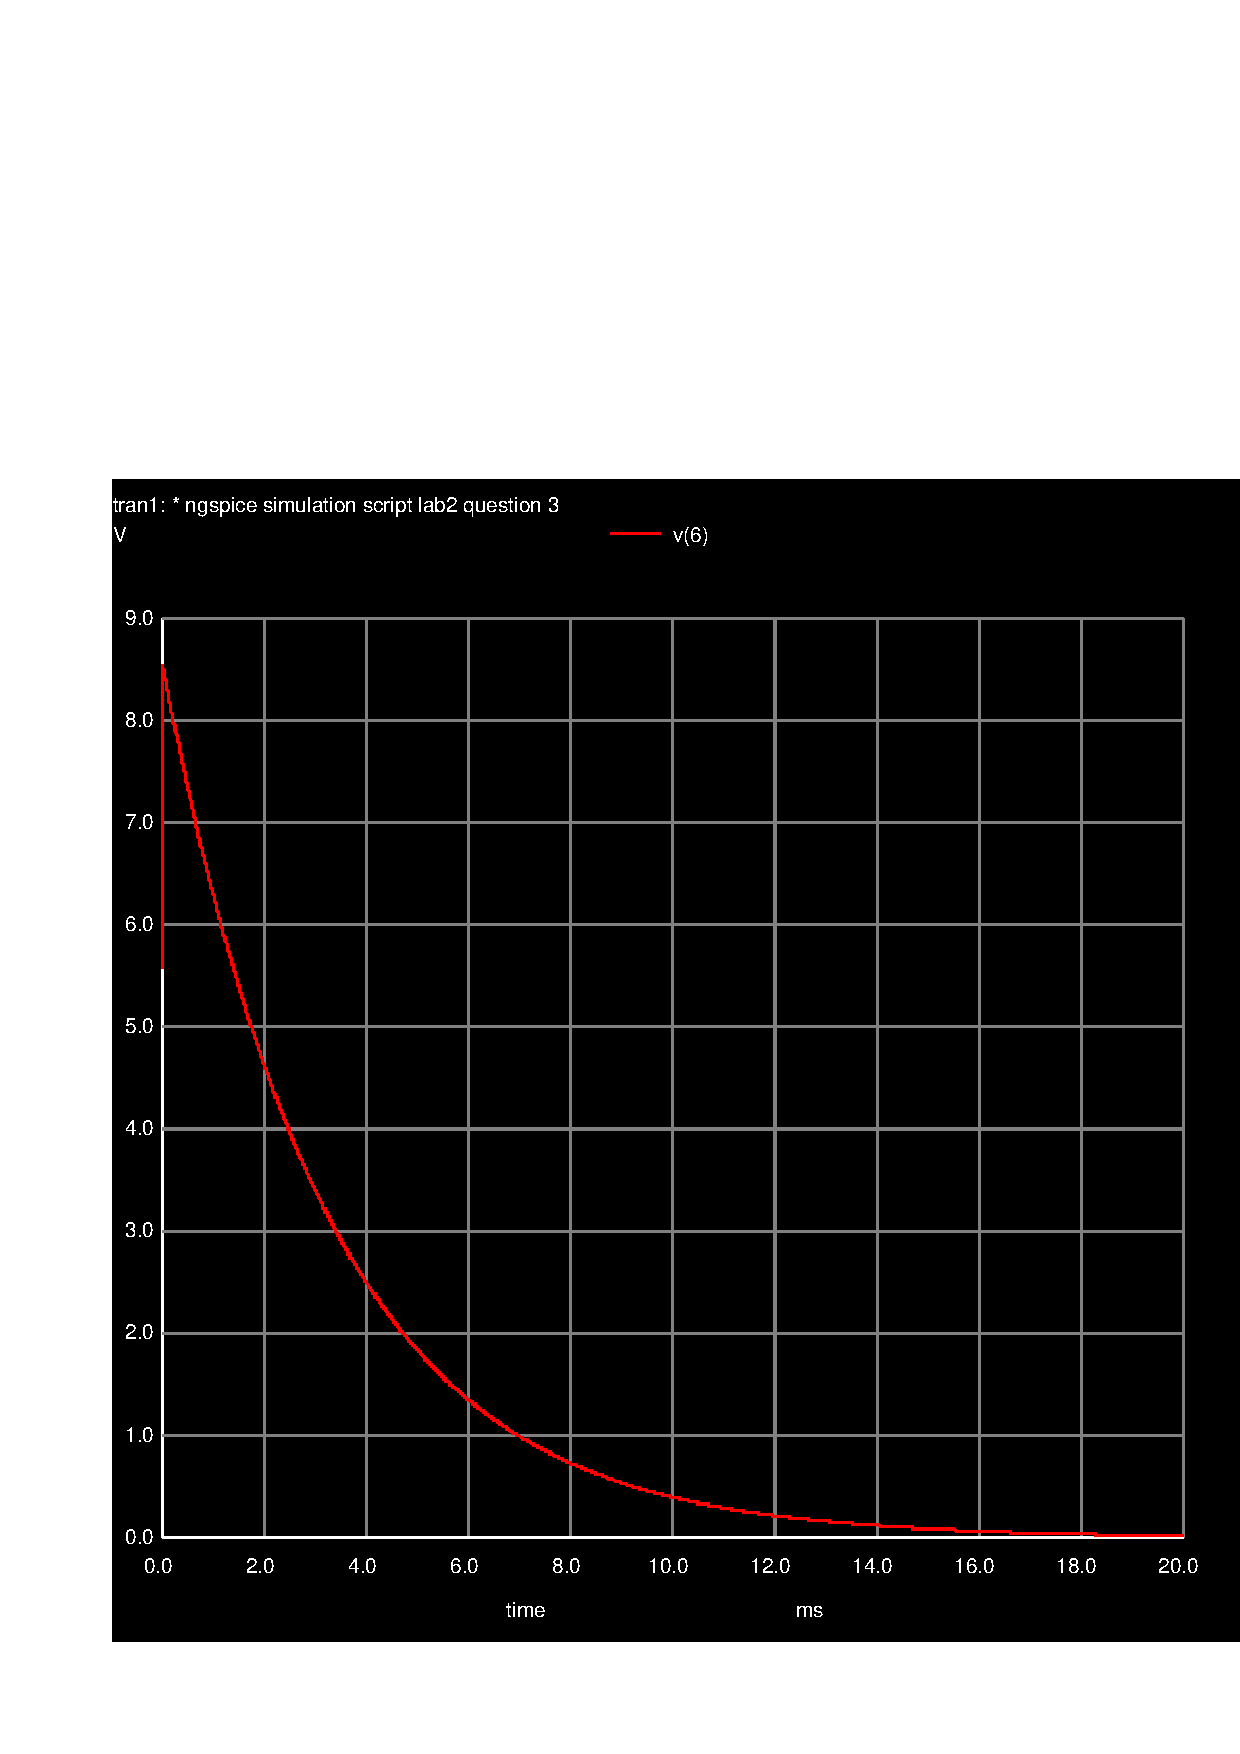
\includegraphics[width=0.7\linewidth]{sim3.pdf}
\caption{Input voltage of the secundary circuit (v(2)), output Voltage of the Envelope Detector (v(4)), Voltage Regulator (v(5)), and v(5)-12}
\label{fig:sim5}
\end{figure}




\begin{figure}[h] \centering
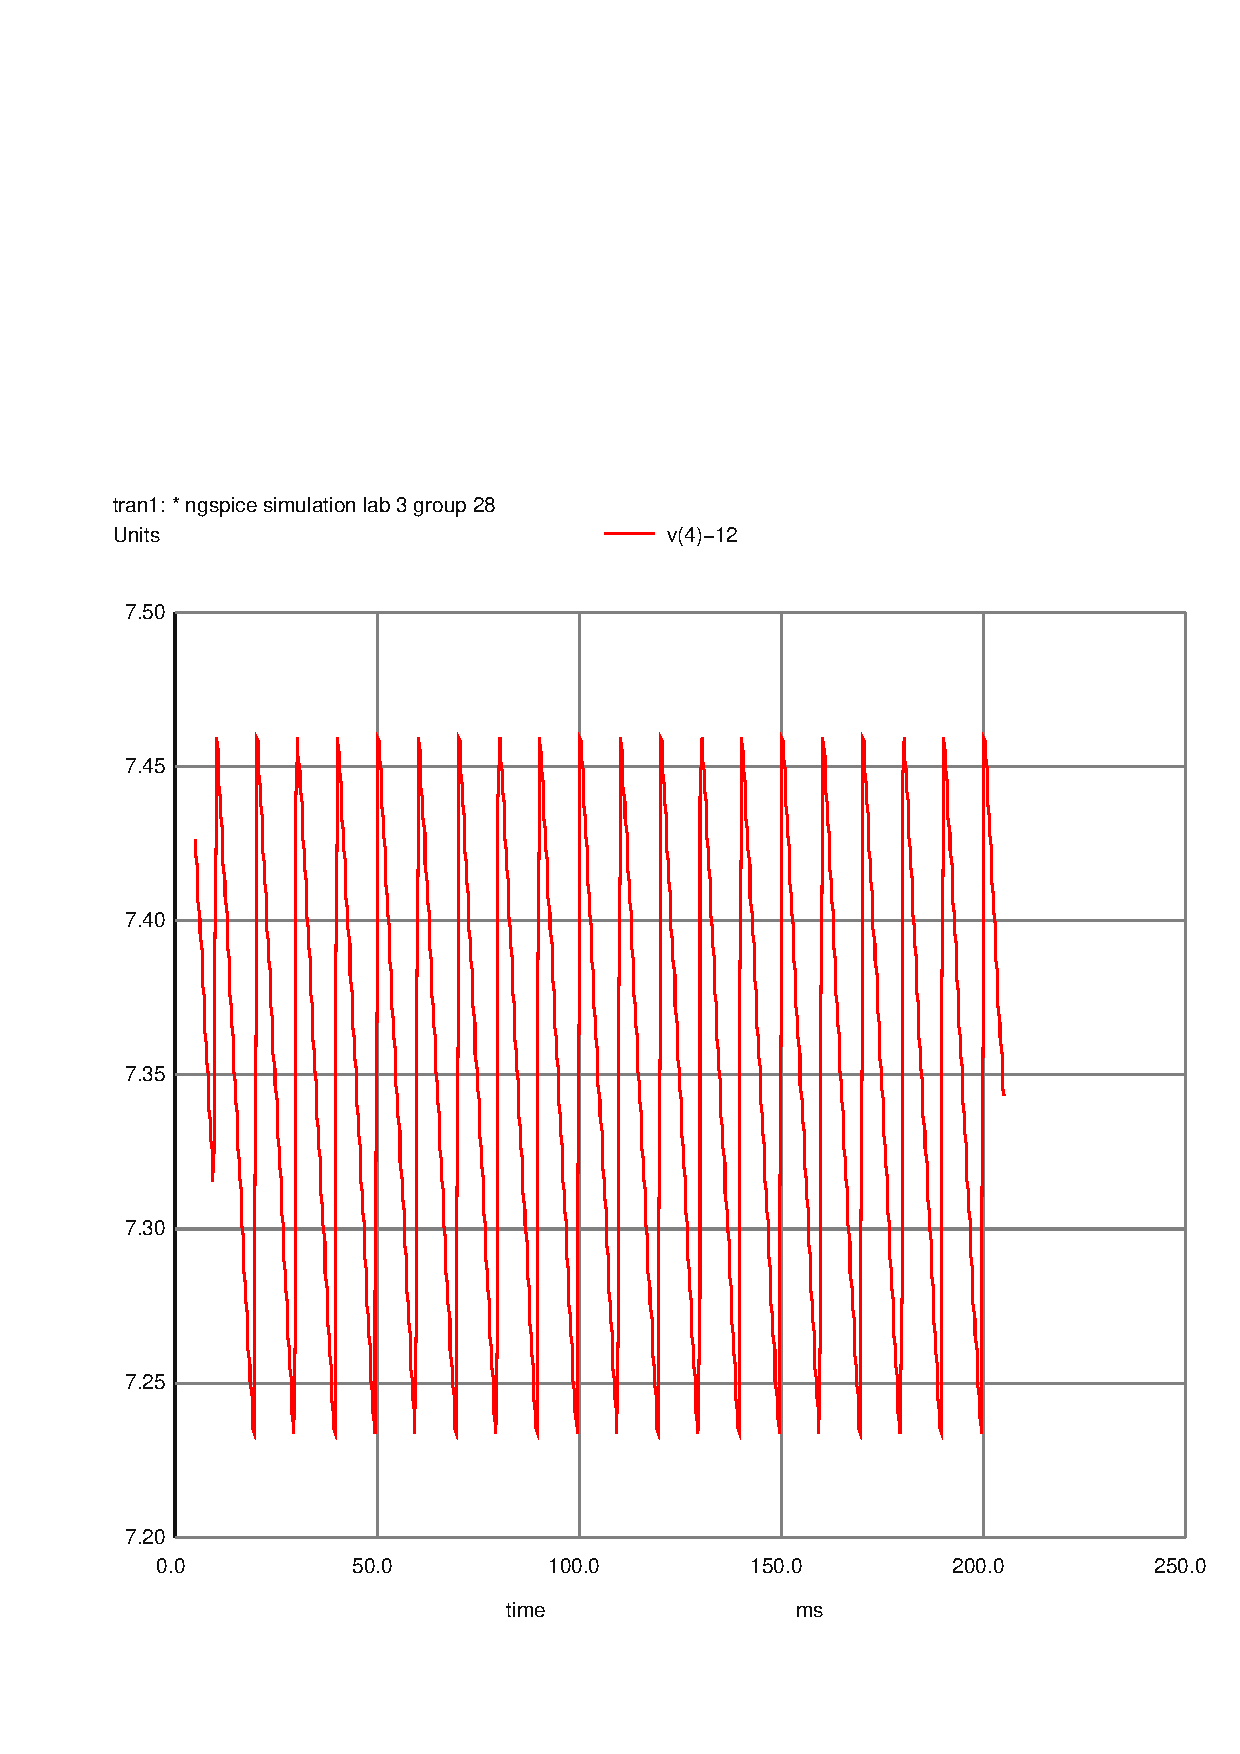
\includegraphics[width=0.7\linewidth]{sim31.pdf}
\caption{Output AC components + DC deviation}
\label{fig:sim5}
\end{figure}


